\chapter{Implementação}
\label{sec:implementacao}

O presente capítulo apresenta a forma como foi estruturado o desenvolvimento do projecto, as técnologias e ferramentas utilizadas e os desafios na implementação. Na secção \ref{sec:ferramentas} são listadas as ferramentas de suporte utilizadas durante o projecto e as técnologias de desenvolvimento. Na secção \ref{sec:sprints} e \ref{sec:dificuldades} estão detalhadas de forma breve todas as sprints planeadas para o projecto e as dificuldades e atrasos no decorrer das mesmas, respectivamente.



\section{Técnologias e Ferramentas Utilizadas}
\label{sec:ferramentas}


\subsection{Ferramentas}

A escolha das ferramentas para o projecto incidiram em dois aspectos: ferramentas utilizadas e impostas pela empresa ou ferramentas utilizadas pelo aluno.

\begin{itemize}
	\item \textbf{VSCode V1.49}\cite{ft1} - \acrfull{ide} de desenvolvimento do projecto. O VSCode é um dos \acrshort{ide} utilizados pela equipa de desenvolvimento da 10.digital e pelo aluno o que facilitou a configuração das convenções de código.
	\item \textbf{draw.io}\cite{ft2} - O draw.io é um editor gráfico que permite aos utilizadores criar e modificar diagramas e gráficos. Esta ferramenta foi utilizada para criar todos os diagramas no decorrer do projecto, inclusive os diagramas presentes neste documento. A decisão da escolha esteve na familiarização com a ferramenta por parte do aluno e também por ser um \textit{software} gratuito e fácil de utilizar.
	\item \textbf{Git V2.24}\cite{ft3} - O Git é um sistema de controlo de versões distribuido, muito utilizado no desenvolvimento de \textit{software}, que regista o historico de alterações. É uma ferramenta utilizada e imposta pela empresa. O Bitbucket\cite{bb} foi serviço de hospedagem utilizado para o repositório online.
	\item \textbf{DBeaver V7.0.1}\cite{ft4} - O DBeaver é um software cliente SQL de administração de base de dados. É um software utilizado pela equipa de desenvolvimento na empresa o que facilitou a escolha visto ter sido apenas para dar suporte ao projecto na fase de desenvolvimento.
	\item \textbf{PostegreSQL V2.3.3e} - Sistema de gestão de base de dados relacionar. Utilizado para a gestão e armazenamento do dados do projecto.
	\item \textbf{Teams}\cite{ft5} - O Teams é a plataforma de comunicação utilizada e imposta pela empresa.
	\item \textbf{Wrike}\cite{ft6} - O Wrike é um \textit{software} de colaboração e gestão de projectos. Esta ferramenta permitiu de forma fácil, gerir e debater sobre cada \textit{sprint} e as tarefas associadas a cada \textit{sprint}. Toda a \textit{scrum team} estava associada ao projecto no wrike, onde, dentro do projecto, estava uma pasta com o \textit{backlog} e uma pasta com todas as reuniões marcadas para gestão do projecto. Na pasta do \textit{backlog} estavam listadas todas as \textit{sprints} planeadas e associada a cada \textit{sprint} estavam os elementos que faziam parte da \textit{sprint} e todas as tarefas necessárias para completar a mesma. Cada tarefa tem um estado associado permitindo à \textins{scrum team} perceber o estado atual do projeto. Os estados utilizados para a gestão das tarefas foram os seguintes:
	\begin{itemize}
		\item \textit{active} - Representa uma tarefa active que ainda se encontra por iniciar.
		\item \textit{in progress} - Representa uma tarefa que está a ser desenvolvida.
		\item \textit{awaiting external approval} - Representa uma tarefa que está à espera de aprovação externa.
		\item \textit{awaiting tests} - Representa uma tarefa aprovada que está pronta para ser testada.
		\item \textit{completed} - Representa uma tarefa que foi concluída.
		\item \textit{cancelled} - Representa uma tarefa que foi cancelada.
	\end{itemize}
	 Esta ferramenta é utilizada e imposta pela empresa. 
\end{itemize}


\subsection{Técnologias}

A escolha das técnologias para o projecto incidiram em dois aspectos: técnologias utilizadas e impostas pela empresa ou experiência da equipa de desenvolvimento e avaliação de técnologias concorrentes.

\subsubsection{Técnologias de Back-end}
\begin{itemize}
	\item \textbf{Django V3.0.4} - \textit{Framework Open-source} para desenvolvimento de aplicações \textit{Web} com python. \textit{Framework} base do servidor. Técnologia utilizada e imposta pela empresa.
	\item \textbf{Python V3.7.3} - Linguagem de programação de alto nível, utilizado para programar o servidor. Técnologia utilizada e imposta pela empresa. Outra condição imposta pela empresa foi o uso da convenção PEP 8\cite{convencao} para todo o código em python.
	\item \textbf{Celery V4.2.1} - O Celery é uma implementação de uma fila de tarefas para aplicações web. Esta técnologia é utilizada para gerir tarefas assincronas no servidor. Técnologia utilizada e imposta pela empresa.
	\item \textbf{plotly V4.8.1} - Biblioteca de python \textit{open-source} que permite criar gráficos interactivos. Esta técnologia foi utilizada para gerar todos os gráficos da secção de analise e tratamentos de dados da plataforma. A empresa actualmente utiliza dois serviços para tratamento e visualização de dados, Power BI\cite{pb} e Superset\cite{bb} que são bastante completos e complexos para  as necessidades do projecto. A visualização dos dados integrada na plataforma é um requisito e neste sentido o Power BI não foi opção. O Superset foi recomendado pela empresa conduto, depois de uma breve análise, o aluno concluiu que o Superset, apesar de permitir a sua integração com a plataforma desenvolvida e ser um serviço bastante completo, que cumpre com os requisitos do projecto, a sua experiência com visualização de dados em python cumpre de igual forma os requisitos do projecto e terá uma curva de aprendizagem muito reduzida dada a familiarização com este tipo de técnologias. 
	Desta forma ambas as técnologias plotly e matplotlib\cite{mpl} seriam opção, mas atentendo às necessidades do projecto, a biblioteca plotly foi escolhida porque ao contrário do matplotlib, permite a criação de gráficos interactivos e uma melhor experiência para o utilizador.
	\item \textbf{Coverage V5.1} - Coverage é uma ferramena (i.e. uma livraria de python) para calcular a cobertura de código em python. Técnologia utilizada para executar testes de cobertura no projeto. Esta técnologia foi recomendade pela empresa.
\end{itemize}

\subsubsection{Técnologias de Front-end}
\begin{itemize}
	\item \textbf{HTML 5.0} - Linguagem utilizada para a construção das páginas \textit{web} da plataforma.
	\item \textbf{JavaScript} - É uma linguagem de programação de alto nível, mais conhecida como linguagem de \textit{scripting} para páginas \textit{web}. Utilizada para execução de \textit{scripts} no lado do cliente, sem ter que passar pelo servidor.
	\item \textbf{jQuery V3.5.1} - Biblioteca de javascript que permite executar pedidos AJAX e manipular facilmente a \acrfull{dom}. 
	\item \textbf{Select2 V4.0.13} - Biblioteca de javascript que disponibiliza um elemento de html (i.e \textit{select box}) costumizável. Esta técnologia facilitou bastante a implementação da seleção de tags na camada de apresentação. Sendo uma técnologia conhecida, com suporte e já tendo sido utilizada pelo aluno foram as razões que incidiram na escolha da técnologia.
	\item \textbf{Bootstrap V4.5.0} - \textit{Framework open-source} de \textit{front-end} que disponibiliza vários componentes de interface para desenvolvimento de aplicações web. Técnologia escolhida pelo \textit{front-end designer} que fez parte da \textit{scrum team}.
\end{itemize}


\section{Desafios na Implementação}
\label{sec:dificuldades}

\subsection{Primeiro Semestre}

Na Figura \ref{fig:gantt2} apresenta-se o plano de estágio relativo ao segundo semestre. A fase de implementação divide-se em várias \textit{sprints}, que serão detalhadas no Capítulo \ref{sec:sprints}.


\begin{figure}[ht!]
	\begin{center}
		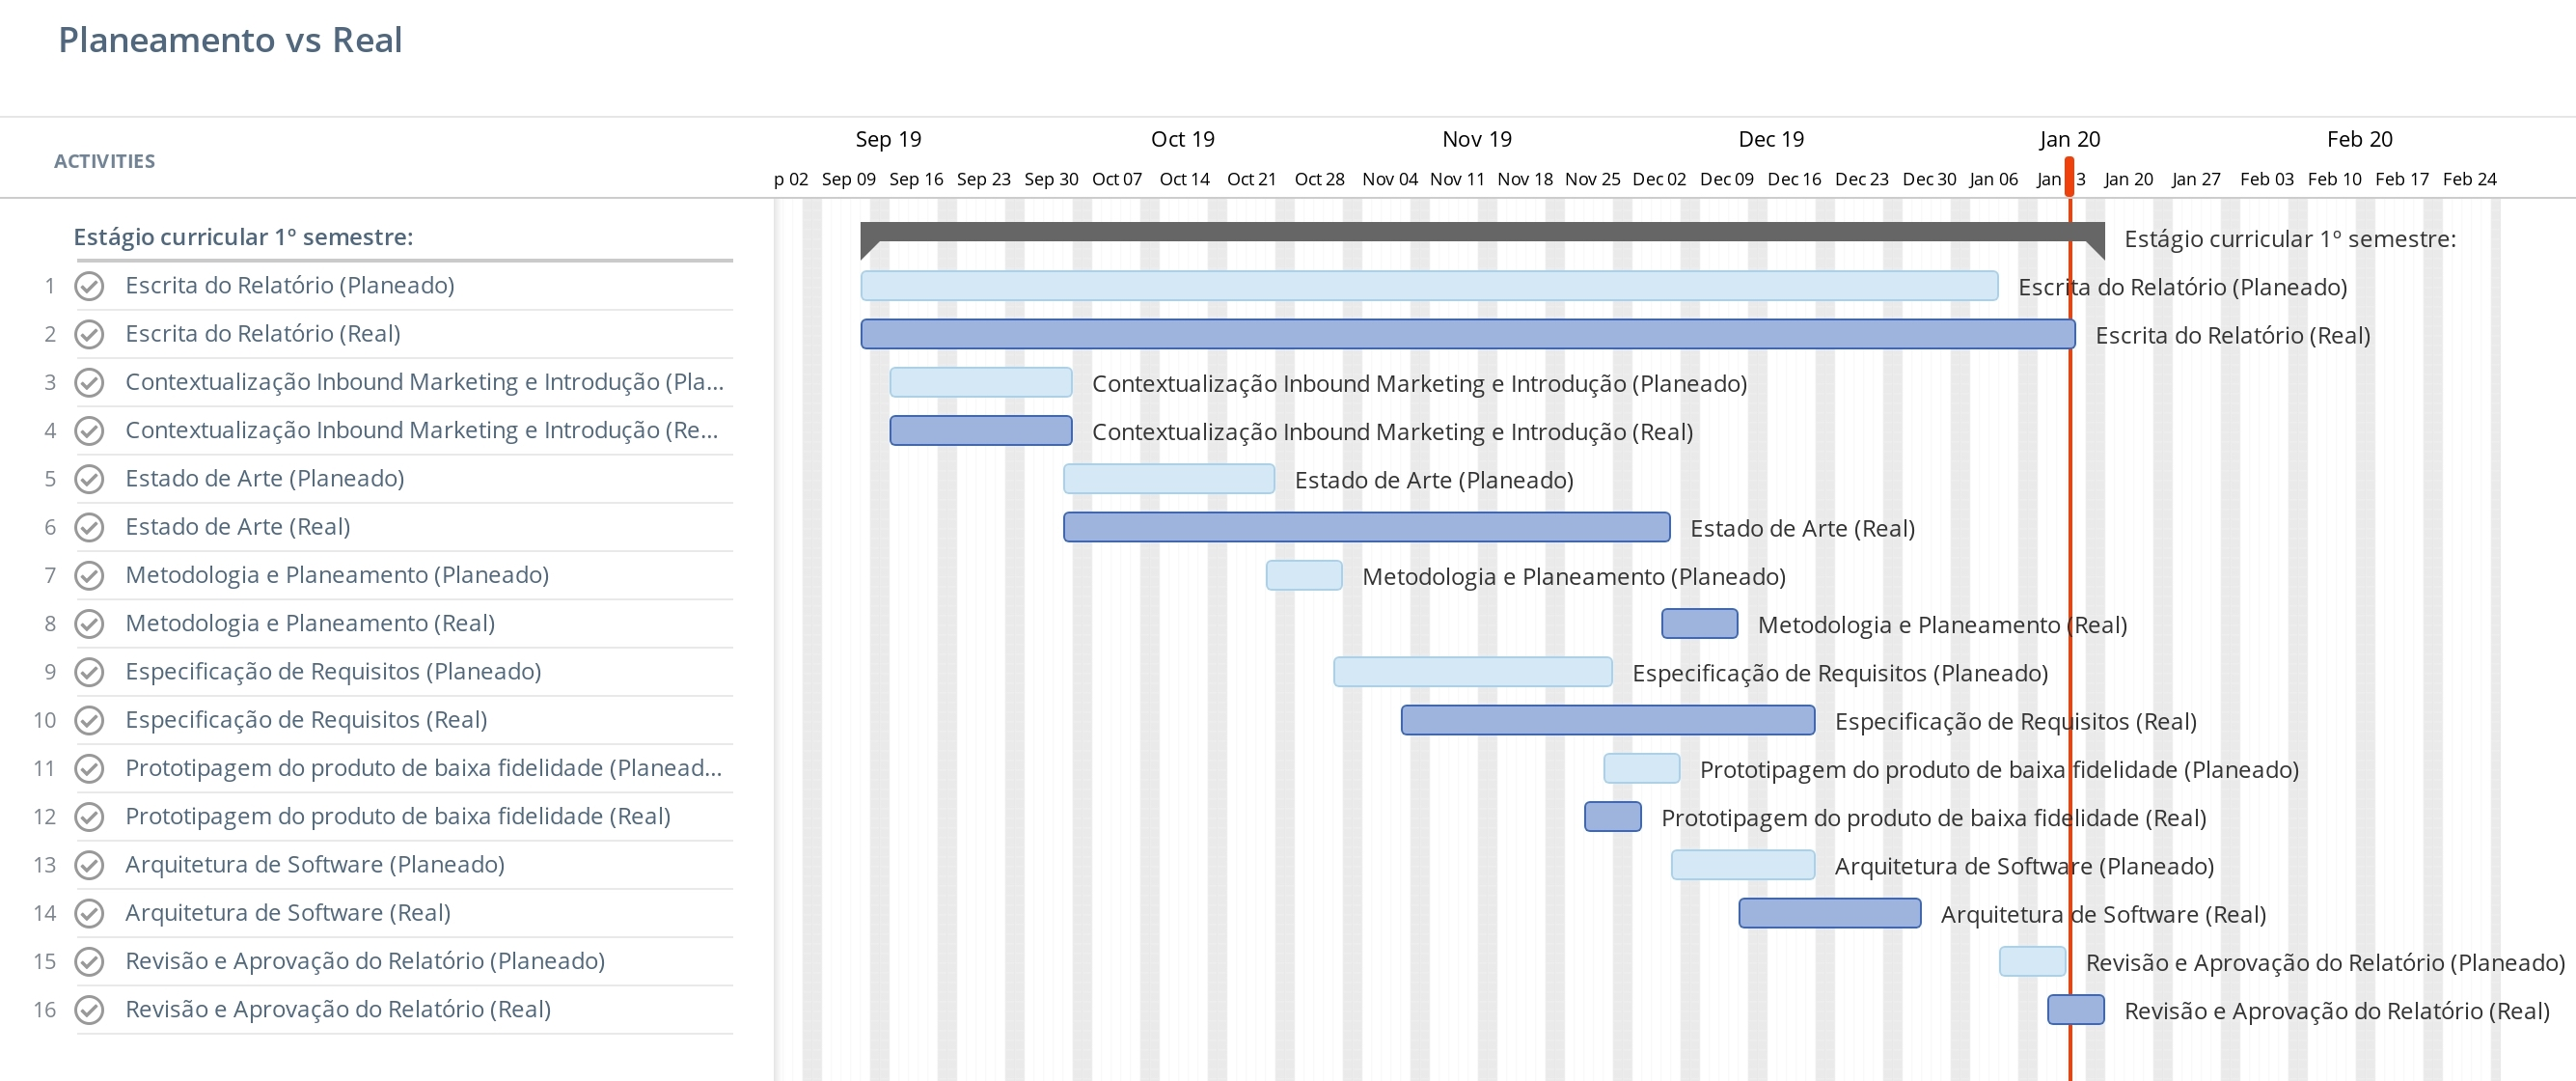
\includegraphics[width=1\textwidth]{img/gantt/vs.jpeg}
		\caption{Diagrama de Gantt - Planeamento vs Real do 1º semestre}
		\label{fig:ganttvs1}
	\end{center}
\end{figure}

Representado na Figura \ref{fig:ganttvs1} temos o planeamento de estágio relativo ao primeiro semestre em comparação com o tempo que o aluno realmente demorou a concluir as tarefas. A primeira tarefa que salta à vista é o Estado de Arte, que claramente excedeu a data limite de entrega para a reunião de ponto com os orientadores de estágio. Um dos fatores decisivos para o atraso na realização da tarefa deveu-se ao facto de ser uma fase de pesquisa e análise do mercado atual, em que é difícil de prever o tempo exato que se demora a realizar esta tarefa. O outro fator decisivo deveu-se ao facto de, a meio do semestre, o cliente ter pedido para implementar uma nova funcionalidade que representa um dos principais objetivos na plataforma a desenvolver. Tudo isto criou um atraso significativo em todas as restantes tarefas. Pode-se também reparar que a escrita da tarefa da Metodologia e Planeamento foi realizada algumas semanas depois do planeado. O aparecimento da nova funcionalidade levou a uma reestruturação do planeamento o que provocou um atraso nesta tarefa, visto que só se iniciou a escrita da mesma depois de ter acabar o novo planeamento.

\subsection{Segundo Semestre}

Como podemos na Figura \ref{fig:plane_2_semestre} , comparando o tempo planeado com o tempo que realmente se demorou a concluir as tarefas consegue-se observar um evelado desvio entre as \textit{sprints}. Nesta secção, é explicado mais ao detalhe os desafios na implementação, que foram a principal causa para os atrasos verificados.

\begin{figure}[ht!]
	\begin{center}
		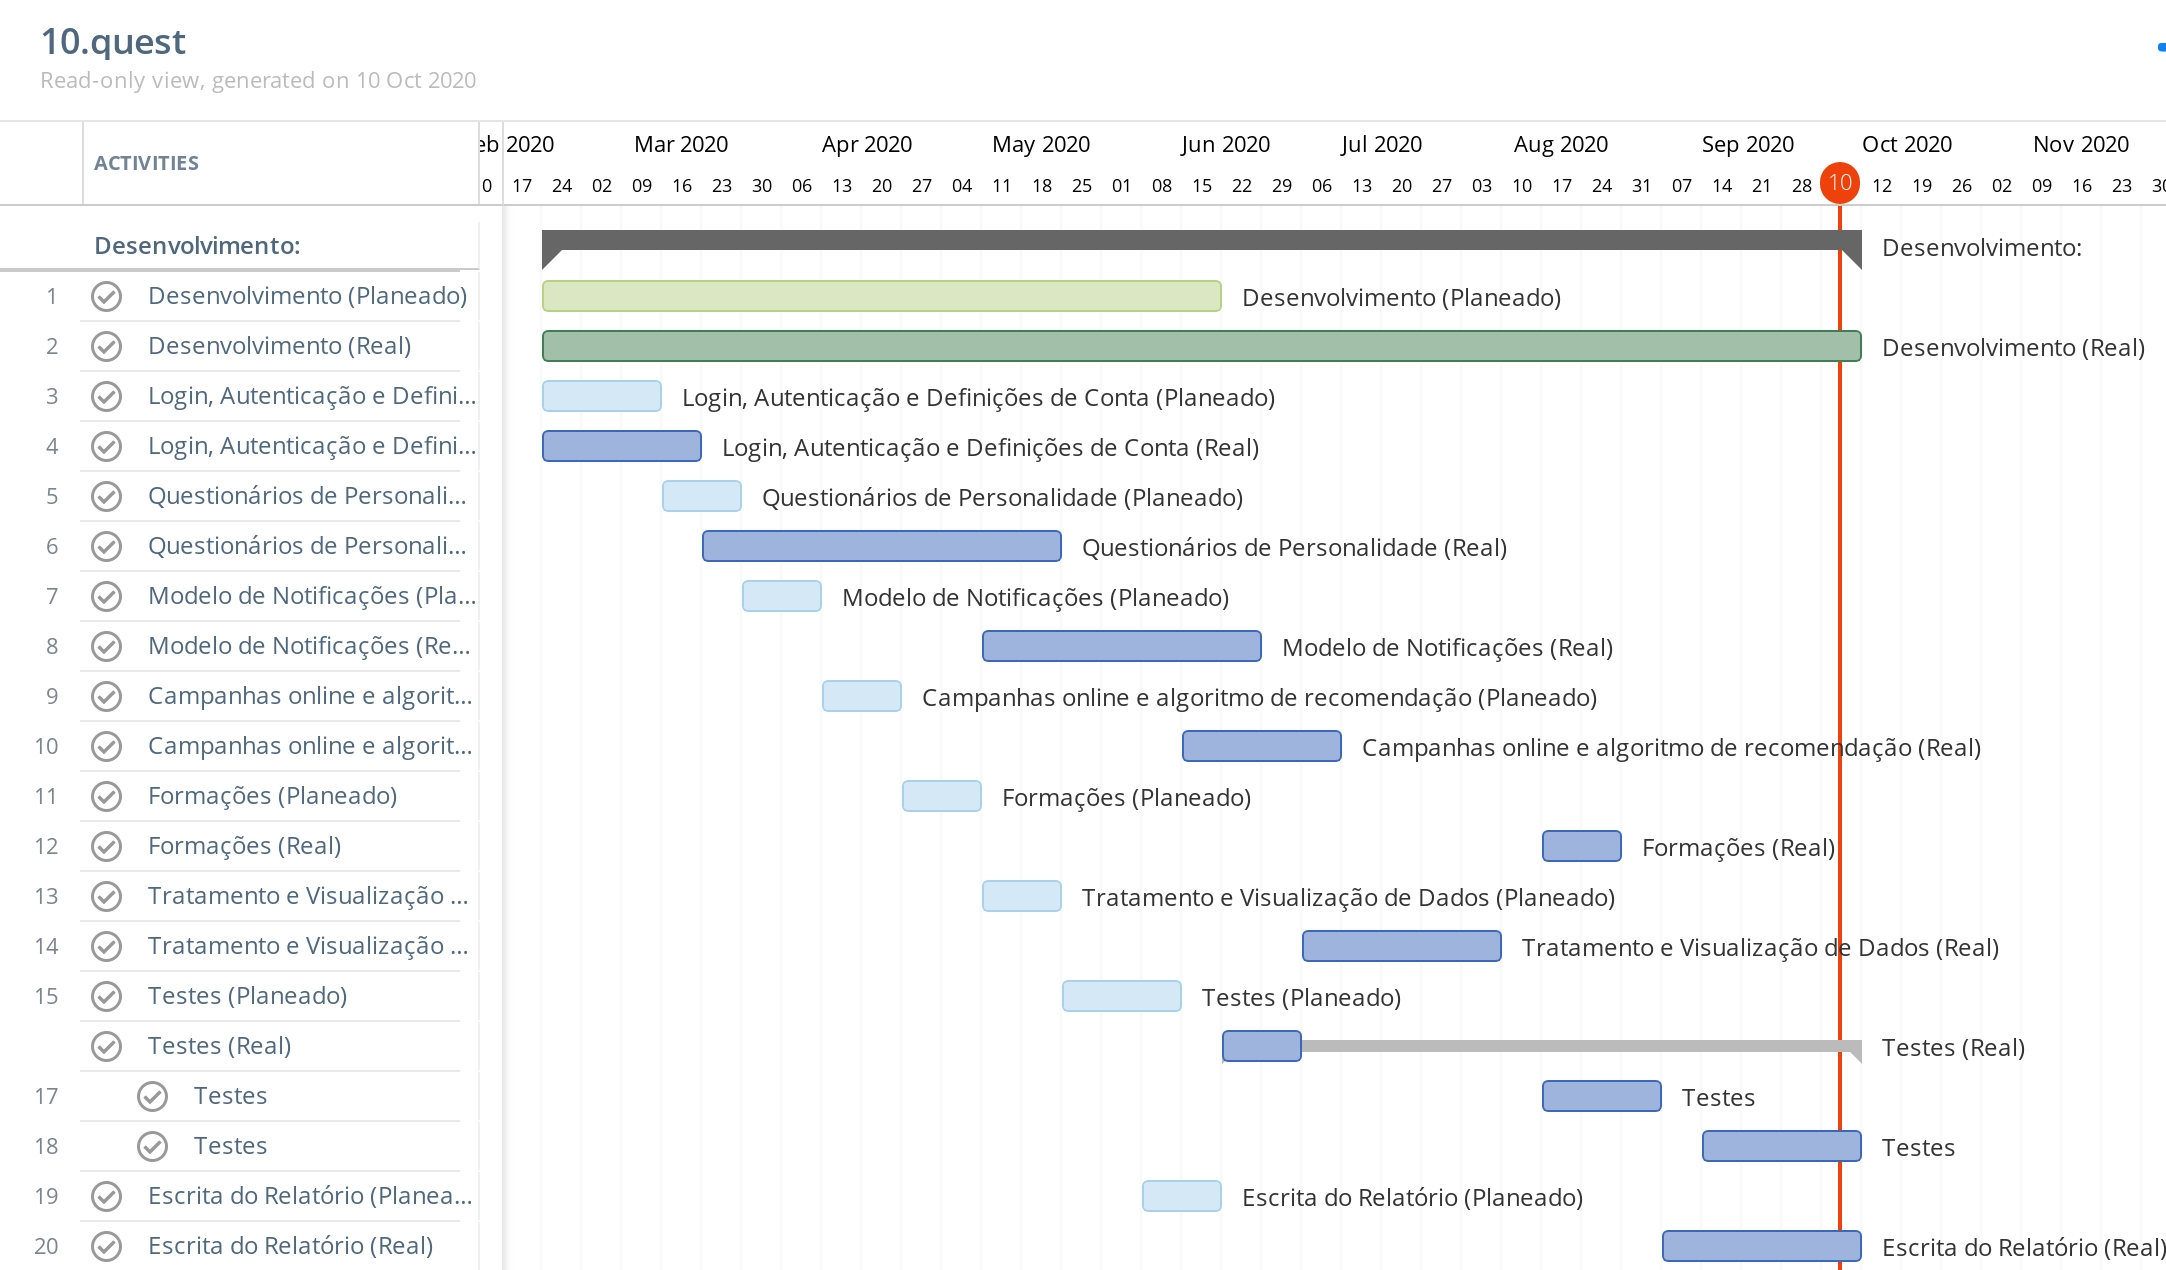
\includegraphics[width=1\textwidth]{img/dev}
		\caption{Planeamento segundo semestre}
		\label{fig:plane_2_semestre}
	\end{center}
\end{figure}

Nesta secção vamos detalhar alguns dos desafios técnologicos que surgiram no decorrer do desenvolvimento do projeto e será também explicado o porquê de terem sido activadas estratégias de mitigação.

A fase de desenvolvimento (i.e. isto é a partir da \textit{sprint \#8}) começou no dia 14 de Feveiro de 2020 e logo nas primeiras \textit{sprints} o aluno sentiu algumas dificuldades em conseguir completar todas as tarefas associadas às diferentes \textit{sprints}. A empresa trabalha com uma serie de técnologias e ferramentas com que o aluno teve que se adaptar rápidamente e foi planeado apenas doze dias para formação interna. Nesta fase o aluno viu-se forçado a activar o plano de mitigação associado ao risco R03 referido na secção \ref{analiseriscos}. Com horas extras de trabalho o aluno conseguiu recuperar algum tempo perdido no projecto e apesar de nunca ter conseguido recuperar na totalidade, manteve o ritmo certo.

Na primeira quinzena de Março a empresa, e todo o grupo onde está inserida, viu-se obrigada a trabalhar remotamente, devido à pandemia que se fez sentir durante o ano, o que teve um impacto directo, negativo, no projeto. A 10.digital (i.e. Dascat Software) trabalha na àrea de marketing e transformação digital, tendo também uma equipa de \textit{e-commerce}, que com a pandemia foram dois sectores (não necessáriamente separados) que registaram um crescimento bastante elevado. 
Para tentar dar resposta ao mercado e acompanhar o crescimento nestes sectores a empresa teve que refazer por completo o plano anual e realucar os recursos às novas necessidades. 
Neste contexto, o desenvolvedor de \textit{front-end} alocado ao projecto para começar a dar apoio na \textit{sprint \#3} foi realucado para dois meses depois. A falta de experiência por parte do aluno em técnologias de \textit{front-end} inicialmente não projudicou o cumprimento das tarefas contudo, numa fase mais adiantada provocou alguns incovenientes. 
Durante a \textit{sprint \#12}, ainda numa fase em que a empresa tentava dar resposta às necessidades do mercado, o desenvolvedor de \textit{front-end} foi alucado ao projecto contudo, seguindo o nove plano anual da empresa, a \textit{scrum team} foi forçada a mudar algumas prioridades associadas aos requisitos funcionais de forma a conseguir reduzir os 20 dias alucados a \textit{front-end} para 8 dias. Isto obrigou o aluno a activar o plano de mitigação associado ao risco R04 referido na secção \ref{analiseriscos}. 

Como foi referido anteriormente, a falta de experiência por parte do aluno em técnologias de \textit{front-end} procovou alguns incovenientes numa fase posterior do projecto. Durante a \textit{sprint \#12} cerca de metade do tempo alucado para desenvolvimento \textit{front-end} acabou por ser gasto a fazer ligação com que estava desenvolvido até ao momento e corrigir problemas de compatibilidade com a nova estrutura de \textit{front-end}. No final da \textit{sprint \#12} apesar de ter sido desenvolvida a estrutura base do \textit{front-end}, nesta fase o aluno viu-se obrigado a continuar com o plano de mitigação associado ao risco R03 referido na secção \ref{analiseriscos}, para conseguir em simultâneo com o desenvolvimento do \textit{back-end}, continuar o desenvolvimento do \textit{front-end}.






\blankpage

\glsresetall
